\documentclass[../main.tex]{subfile}

\begin{document}

\topictitle{Basics}

\sectitle{Definitions}

\begin{figure}[h]
\begin{minipage}{0.6\linewidth}
\centering
\resizebox{0.8\linewidth}{!}{%
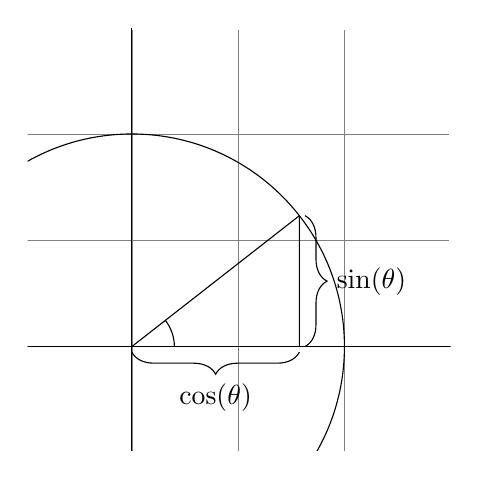
\begin{tikzpicture}[scale=2.7]
	\clip (1.5,1.5) rectangle (-0.49,-0.49);

	\coordinate (O) at (0,0);
	\coordinate (P) at (38:1);
	\coordinate (I) at (P |- O);

	\draw [step=0.5, gray, ultra thin] (1.49,1.49) grid (-1.49,-1.49);

	\draw (-1.5,0) -- (1.5,0) (0,1.5) -- (0,-1.5);
	\draw (0,0) circle[radius=1];

	\draw (0,0) -- (P);
	\draw (P) -- (I);

	\draw (0.2,0) arc[start angle=0, end angle=38, radius=0.2];
	%\draw (0.1,0) node [anchor=south west] {$\theta$};

	\draw [decorate, decoration={brace, amplitude=8pt, raise=2pt}] (P) -- node [right, xshift=10pt] {$\sin(\theta)$} (I);
	\draw [decorate, decoration={brace, amplitude=8pt, mirror, raise=2pt}] (O) -- node [below, yshift=-10pt] {$\cos(\theta)$} (I);
\end{tikzpicture}
}\end{minipage}\hspace{3ex}
\begin{minipage}{0.25\linewidth}
	\large
	\begin{empheq}[box=\rememberBox]{align*}
		\tan\theta &\equiv \frac{\sin\theta}{\cos\theta}\\[1.5ex]
		\sec\theta &\equiv \frac{1}{\cos\theta}\\[1.5ex]
		\cosec\theta &\equiv \frac{1}{\sin\theta}\\[1.5ex]
		\cot\theta &\equiv \frac{1}{\tan\theta} \equiv \frac{\cos\theta}{\sin\theta}
	\end{empheq}
\end{minipage}
\end{figure}

\vspace{2ex}
\sectitle{Identities}

{\large
\begin{empheq}[box=\rememberBox]{alignat*=3}
	\sin^2\theta + \cos^2\theta &\equiv 1\ \ \ \ \ &
	1 + \tan^2\theta &\equiv \sec^2\theta\ \ \ \ \ &
	1 + \cot^2\theta &\equiv \cosec^2\theta
\end{empheq}
}

\begin{figure}[H]
\large
\begin{minipage}{0.49\linewidth}
	\begin{empheq}[box=\formulaBookBox]{align*}
		\sin(\alpha \pm \beta) &\equiv \sin\alpha\cos\beta \pm \cos\alpha\sin\beta\\[2ex]
		\cos(\alpha \pm \beta) &\equiv \cos\alpha\cos\beta \mp \sin\alpha\sin\beta\\[2ex]
		\tan(\alpha \pm \beta) &\equiv \frac{\tan\alpha \pm \tan\beta}{1 \mp \tan\alpha\tan\beta}
	\end{empheq}
\end{minipage}\hfill
\begin{minipage}{0.49\linewidth}
	\begin{empheq}[box=\rememberBox]{align*}
		\sin 2\theta &\equiv 2\sin\theta\cos\theta\\[2ex]
		\tan 2\theta &\equiv \frac{2\tan\theta}{1 - \tan^2\theta}\\[2ex]
		\cos 2\theta &\equiv \cos^2\theta - \sin^2\theta\\
			&\equiv 2\cos^2\theta - 1\\
			&\equiv 1 - 2\sin^2\theta
	\end{empheq}
\end{minipage}
\end{figure}

\end{document}
